\documentclass{beamer}
\usetheme{Madrid}
\usepackage[T1]{fontenc}
\usepackage{mathpazo}
\usepackage{graphicx}
\usepackage{booktabs}
\usepackage{tikz}
\usetikzlibrary{positioning,arrows.meta,shapes.geometric,fit,backgrounds,calc}
\definecolor{cetnavy}{RGB}{10,26,63}
\definecolor{cetlight}{RGB}{225,231,242}
\setbeamercolor{structure}{fg=cetnavy}
\setbeamercolor{frametitle}{bg=cetnavy,fg=white}
\setbeamercolor{title}{bg=cetnavy,fg=white}
\setbeamertemplate{navigation symbols}{}
% =====================================================================
%  EDIT YOUR DETAILS HERE — this ONE file feeds every abstract & deck.
%  (Change a value, recompile; all 36 documents update.)
% =====================================================================
\newcommand{\seminarName}{Aflah Muhammed P}      % <-- your full name (guessed from your email; please verify)
\newcommand{\seminarRoll}{TVE00CS000}            % <-- your university register/roll number
\newcommand{\seminarClassRoll}{00}               % <-- your class roll no (the short one)
\newcommand{\seminarGuide}{Prof.\ <Guide Name>}  % <-- your guide
\newcommand{\seminarDept}{Department of Computer Science and Engineering}
\newcommand{\seminarCollege}{College of Engineering Trivandrum}
\newcommand{\seminarShortCollege}{CET}           % shown in the slide footer, e.g. "Aflah Muhammed P (CET)"
\newcommand{\seminarShortTitle}{B.Tech Seminar}  % middle of the slide footer
\newcommand{\seminarDate}{July 31, 2026}
% ---------------------------------------------------------------------
% Optional: put a logo image named  cet_logo.png  in this folder and it
% will appear on every title slide automatically. If absent, it is skipped.
% =====================================================================

\title[\seminarShortTitle]{The Berkeley Function-Calling Leaderboard: Benchmarking Tool Use}
\author[\seminarName\ (\seminarShortCollege)]{\seminarName \\ \seminarRoll \\ Roll No: \seminarClassRoll \\ Guide: \seminarGuide}
\institute[\seminarShortCollege]{\seminarDept \\ \seminarCollege}
\date{\seminarDate}
\titlegraphic{\IfFileExists{cet_logo.png}{\includegraphics[height=1.1cm]{cet_logo.png}}{}}
\begin{document}
\begin{frame}\titlepage\end{frame}
\begin{frame}{Table of Contents}\tableofcontents\end{frame}
\section{Introduction}
\begin{frame}{What is Function Calling?}
\textbf{\textit{Tool use is core to agentic LLMs}}
\begin{itemize}
\item LLMs invoke external functions, APIs, and tools.
\item Powers agents, plugins, and automation pipelines.
\item Requires correct name, arguments, and types.
\item No standard benchmark existed to measure it.
\item BFCL fills this gap for the community.
\end{itemize}
\end{frame}

\begin{frame}{The Berkeley Function-Calling Leaderboard}
\begin{itemize}
\item Public benchmark and live leaderboard.
\item Execution-free scoring via AST matching.
\item Spans single-turn calls to multi-turn agents.
\item Now a de-facto standard for tool use.
\item ICML 2025; from Gorilla / Berkeley Sky Lab.
\end{itemize}
\end{frame}

\section{Literature Survey}
\begin{frame}{Prior Work on Tool Use}
\textbf{\textit{Related benchmarks and systems}}
\begin{itemize}
\item Gorilla: LLM fine-tuned to write API calls.
\item ToolLLM / ToolBench: 16000+ real-world APIs.
\item API-Bank, Nexus, ToolEval: tool-use datasets.
\item Most cover only single-call scenarios.
\item Often narrow, contamination-prone, execution-heavy.
\end{itemize}
\end{frame}

\section{Motivation}
\begin{frame}{Why a New Benchmark?}
\begin{itemize}
\item Judging call validity is genuinely hard.
\item Executable checks need live, brittle APIs.
\item Diverse real-world functions are scarce.
\item Data contamination inflates reported scores.
\item Field is shifting from tool use to agents.
\end{itemize}
\end{frame}

\section{Problem Statement}
\begin{frame}{The Core Problem}
\begin{itemize}
\item No standard, scalable measure of function calling.
\item Must handle single, parallel, and multiple calls.
\item Must reward abstention when no function fits.
\item Must test stateful, multi-turn agentic behaviour.
\item Should avoid costly live execution.
\end{itemize}
\end{frame}

\section{Objectives}
\begin{frame}{Goals and Contributions}
\begin{itemize}
\item AST metric scaling to thousands of functions.
\item Coverage across multiple programming languages.
\item Categories from simple calls to agentic tasks.
\item Live, user-contributed data to curb contamination.
\item An open, continuously updated leaderboard.
\end{itemize}
\end{frame}

\section{Methodology Overview}
\begin{frame}{AST Matching Pipeline}
\begin{center}
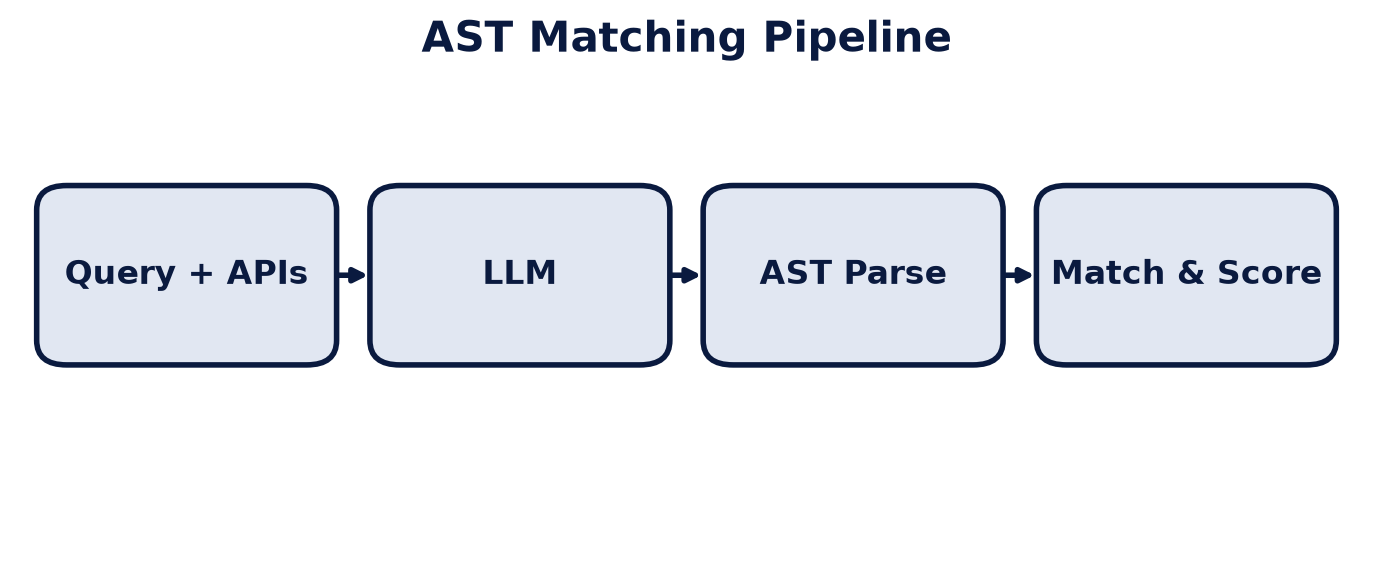
\includegraphics[width=0.9\textwidth,height=0.62\textheight,keepaspectratio]{images/bfcl_1.png}
\end{center}
\begin{itemize}
\item Parse predicted call into a syntax tree.
\item Compare against ground-truth structure; no execution.
\end{itemize}
\end{frame}

\section{System Architecture}
\begin{frame}{Four Evaluation Tracks}
\begin{center}
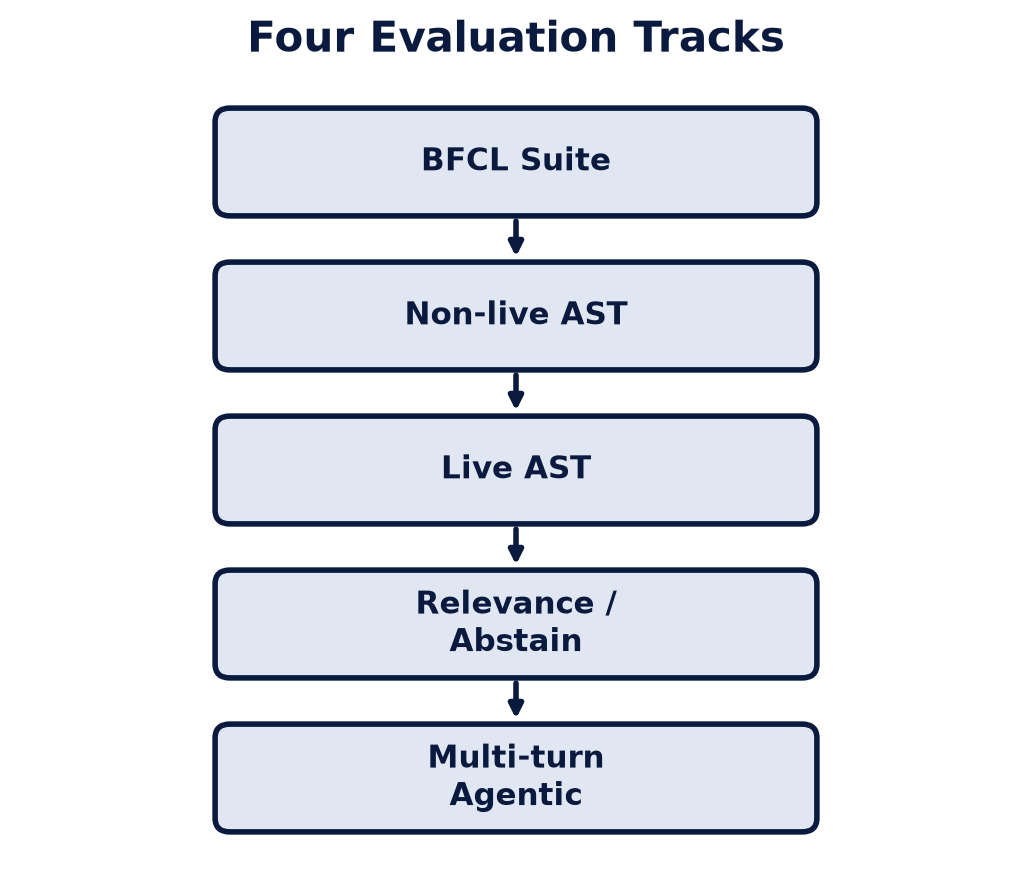
\includegraphics[width=0.9\textwidth,height=0.62\textheight,keepaspectratio]{images/bfcl_2.png}
\end{center}
\begin{itemize}
\item Expert-curated static and live user prompts.
\item Abstention and stateful multi-turn tasks.
\end{itemize}
\end{frame}

\section{Data Collection}
\begin{frame}{Datasets and Categories}
\textbf{\textit{Expert-curated non-live set}}
\begin{itemize}
\item Simple (400), multiple, parallel, parallel-multiple (200 each).
\item Languages: Python, Java, JavaScript, and REST.
\end{itemize}
\textbf{\textit{Live and agentic sets}}
\begin{itemize}
\item Live prompts contributed by real users.
\item Multi-turn scenarios test memory and state.
\end{itemize}
\end{frame}

\section{Model Development}
\begin{frame}{Scoring Algorithm}
\textbf{\textit{Single-turn AST check}}
\begin{itemize}
\item Verify function name and required parameters.
\item Match value ranges and argument types.
\item Relevance: reward no call when irrelevant.
\end{itemize}
\textbf{\textit{Multi-turn evaluation}}
\begin{itemize}
\item State-based checks for write operations.
\item Augmented: missing function, missing parameter, long context.
\end{itemize}
\end{frame}

\section{Results}
\begin{frame}{Single-turn vs Multi-turn}
\begin{center}
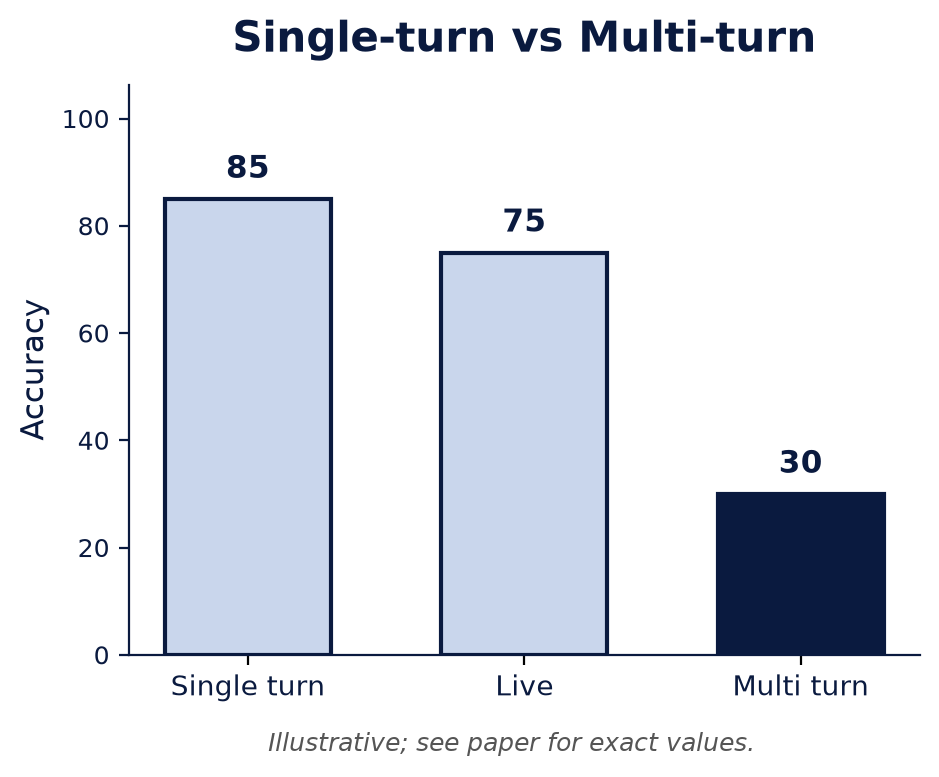
\includegraphics[width=0.9\textwidth,height=0.62\textheight,keepaspectratio]{images/bfcl_3.png}
\end{center}
\begin{itemize}
\item Overall score: unweighted average of sub-categories.
\item Models strong single-turn, much weaker multi-turn.
\end{itemize}
\end{frame}

\section{Discussions}
\begin{frame}{Why AST Matching Works}
\begin{itemize}
\item Execution-free: no live API or sandbox needed.
\item Scales to thousands of diverse functions.
\item Reproducible and cheap across languages.
\item Live data reduces contamination over time.
\item Trade-off: cannot catch some runtime semantics.
\end{itemize}
\end{frame}

\section{Challenges}
\begin{frame}{Open Limitations}
\begin{itemize}
\item Memory retention across long dialogues is weak.
\item Dynamic decision-making remains unreliable.
\item Long-horizon multi-step reasoning still fails.
\item AST misses some execution-time errors.
\item Reliable abstention is hard for models.
\end{itemize}
\end{frame}

\section{Future Work}
\begin{frame}{Directions Ahead}
\begin{itemize}
\item Extend to agentic web search and memory.
\item Study prompt and format sensitivity.
\item Add harder long-horizon, stateful tasks.
\item Broaden language and API coverage.
\item Keep the leaderboard continuously refreshed.
\end{itemize}
\end{frame}

\section{Conclusion}
\begin{frame}{Conclusion}
\begin{itemize}
\item BFCL standardises function-calling evaluation.
\item AST matching is scalable and execution-free.
\item Categories span tool use to agentic tasks.
\item Single-turn is largely solved; multi-turn is open.
\item A de-facto benchmark guiding future tool-use LLMs.
\end{itemize}
\end{frame}

\section{References}
\begin{frame}{References}
\footnotesize
\begin{itemize}
\item S. G. Patil, H. Mao, F. Yan, C. Ji, V. Suresh, I. Stoica, and J. E. Gonzalez, ``The Berkeley Function Calling Leaderboard (BFCL): From Tool Use to Agentic Evaluation of Large Language Models,'' in Proc. ICML, PMLR, vol. 267, 2025.
\item S. G. Patil, T. Zhang, X. Wang, and J. E. Gonzalez, ``Gorilla: Large Language Model Connected with Massive APIs,'' arXiv:2305.15334, 2023.
\item Y. Qin et al., ``ToolLLM: Facilitating Large Language Models to Master 16000+ Real-world APIs,'' in Proc. ICLR, 2024.
\end{itemize}
\end{frame}
\begin{frame}\vfill\centering{\Huge Thank You}\vfill\end{frame}
\end{document}
